% flashcards-title: Sighting a floating pointer from three eye positions
% flashcards-desc: A horizontal scale has labeled marks at twenty, thirty, and forty with equal small steps between them. The tip of a pointer floats a short distance above the scale, directly over the thirty mark. Well above the scale sit three drawn eyes: one to the left, one directly above the pointer tip, and one to the right. From each eye a dashed sight line passes through the pointer tip and continues down to the scale, meeting it at three different points marked with dots labeled a, b, and c from left to right.
\documentclass[dvisvgm,tikz,border=8pt]{standalone}
\usepackage{tikz}
\usetikzlibrary{arrows.meta,calc,positioning}
\definecolor{DeckInk}{HTML}{172A3A}
\definecolor{DeckAccent}{HTML}{176B87}
\definecolor{DeckWarm}{HTML}{D97706}
\definecolor{DeckMuted}{HTML}{667784}
\definecolor{DeckPaper}{HTML}{F7FAFC}
\tikzset{
  every node/.style={font=\sffamily, text=DeckInk},
  object/.style={draw=DeckInk, line width=1.1pt, fill=DeckPaper},
  primary/.style={draw=DeckAccent, line width=1.5pt},
  boundary/.style={draw=DeckAccent, line width=1.5pt, dashed, rounded corners=6pt},
  guide/.style={draw=DeckMuted, line width=0.9pt, dashed},
  dimension/.style={{Stealth[length=3.2mm,width=2.2mm]}-{Stealth[length=3.2mm,width=2.2mm]}, draw=DeckWarm, line width=1.2pt},
  motion/.style={-{Stealth[length=3.5mm,width=2.5mm]}, draw=DeckAccent, line width=1.5pt, dashed},
}

\begin{document}
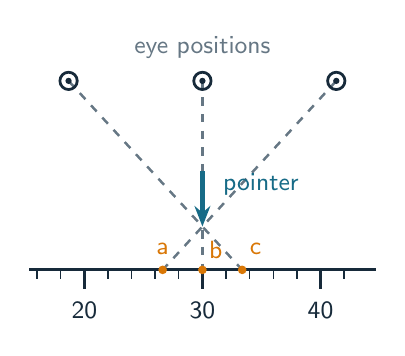
\begin{tikzpicture}[x=1cm,y=1cm]
  % Sight lines first, so the pointer and dots paint over them
  \draw[guide] (-1.7,2.4) -- (0.505,0);
  \draw[guide] (0,2.4) -- (0,0);
  \draw[guide] (1.7,2.4) -- (-0.505,0);
  % Scale
  \draw[DeckInk, line width=1.1pt] (-2.2,0) -- (2.2,0);
  \foreach \x in {-2.1,-1.8,...,2.1}
    \draw[DeckInk, line width=0.5pt] (\x,0) -- (\x,-0.12);
  \foreach \x/\v in {-1.5/20, 0/30, 1.5/40}{
    \draw[DeckInk, line width=0.9pt] (\x,0) -- (\x,-0.24);
    \node[font=\sffamily\small] at (\x,-0.52) {\v};
  }
  % Pointer ending above the scale
  \draw[primary,-{Stealth[length=2.6mm,width=2.0mm]}] (0,1.25) -- (0,0.55);
  \node[text=DeckAccent, font=\sffamily\small, anchor=west] at (0.14,1.08) {pointer};
  % Eyes
  \foreach \x in {-1.7,0,1.7}{
    \draw[DeckInk, line width=1.0pt] (\x,2.4) circle (0.11);
    \fill[DeckInk] (\x,2.4) circle (0.04);
  }
  \node[text=DeckMuted, font=\sffamily\small] at (0,2.82) {eye positions};
  % Apparent reading points
  \fill[DeckWarm] (-0.505,0) circle (0.055);
  \fill[DeckWarm] (0,0) circle (0.055);
  \fill[DeckWarm] (0.505,0) circle (0.055);
  \node[text=DeckWarm, font=\sffamily\small] at (-0.505,0.26) {a};
  \node[text=DeckWarm, font=\sffamily\small] at (0.17,0.26) {b};
  \node[text=DeckWarm, font=\sffamily\small] at (0.675,0.26) {c};
\end{tikzpicture}
\end{document}
